% !TeX program = XeLaTeX
% !TeX encoding = UTF-8
% nikachu2012 default TeX template v1.4
% Compiler : XeLaTeX
% TeX ver  : TeX Live 2023
\documentclass[a4paper, xelatex, ja=standard, 10.5pt]{bxjsarticle}
\setpagelayout*{top=25truemm,bottom=25truemm,left=25truemm,right=25truemm}
\addtolength{\headsep}{\topskip}
\setlength{\headsep}{15pt}
\setlength{\footskip}{30pt}

% パッケージインストール
\usepackage{plisting}
\usepackage{docmute}

% 文書開始
\begin{document}

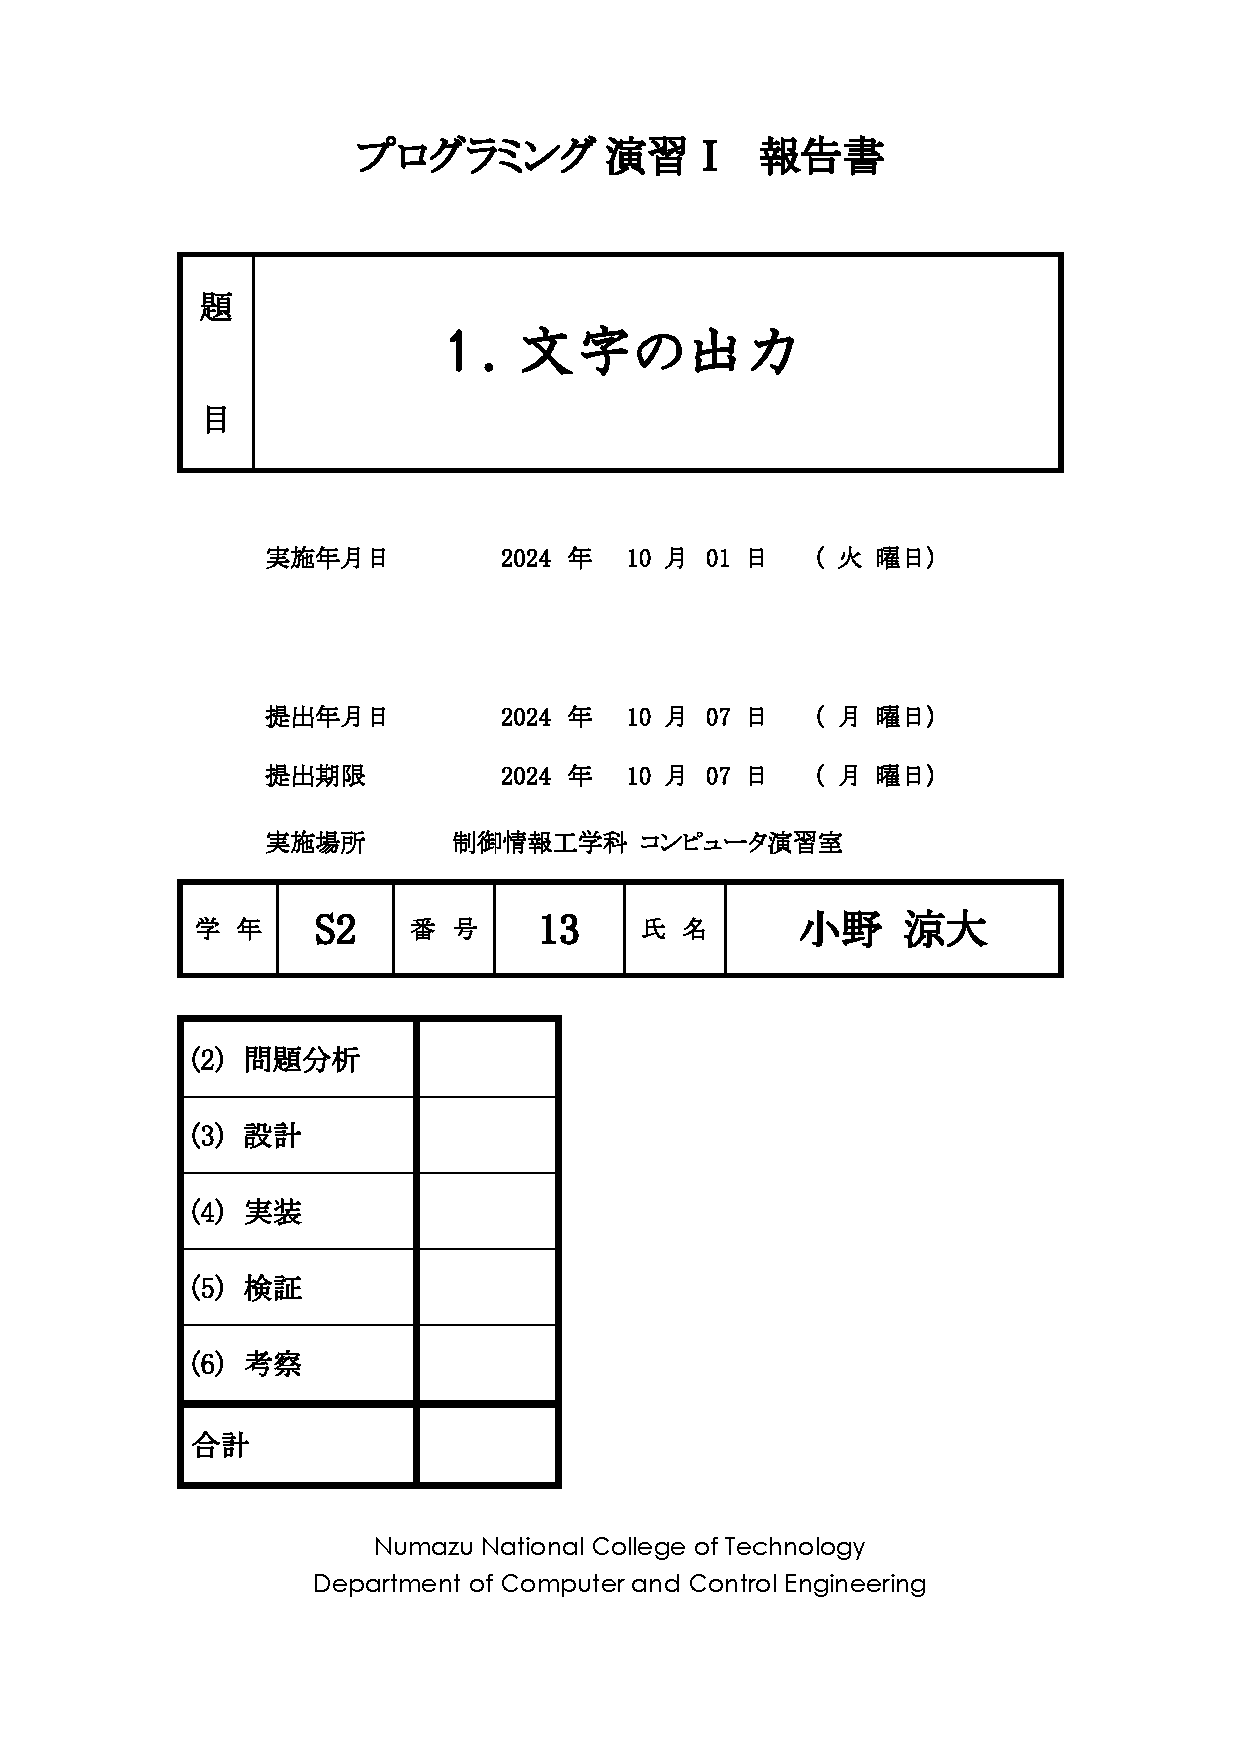
\includepdf{cover.pdf}

\section{問題設定}
\begin{lstlisting}
Hello.
私は小野です。
\end{lstlisting}
という2行のメッセージを画面に表示する.

\section{問題分析}
今回の問題はターミナル上に英語と日本語のメッセージを表示させれば良い.
まず「\texttt{Hello.}」と半角英語で表示して改行し,
次に「\texttt{私は小野です。}」と全角日本語で表示して改行する.
そしてプログラムを終了させれば良い.

本プログラム作成にあたり,
標準入出力(stdard input output)ヘッダファイルの\texttt{<stdio.h>},
文字列を表示する\texttt{printf},
改行の制御文字\texttt{\textbackslash n}を用いる.

\section{設計}
以下に今回作成するプログラムのフローチャートを示す.

\begin{figure}[H]
\centering
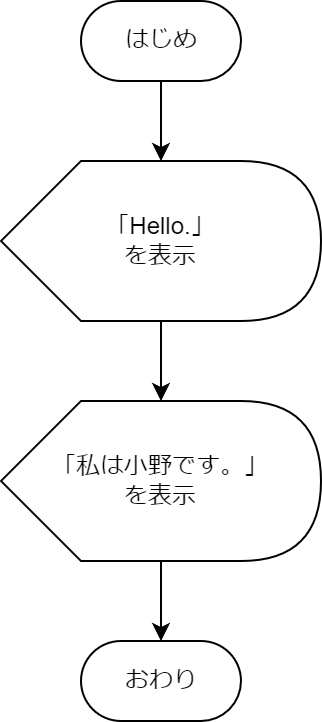
\includegraphics[scale=0.5]{img/flowchart.drawio.png}
\caption{フローチャート}
\label{}
\end{figure}

\section{実装}
まず今回書いたコードを載せる.
\begin{lstlisting}[caption=ソースコード,label=s01]
/*************************************************
例題1 メッセージの表示[ex01.c]
**************************************************/

#include <stdio.h> // standard input output ヘッダを読み込む

int main(void) // main関数のはじまり
{
    printf("Hello.\n");         // "Hello."を表示
    printf("私は小野です。\n"); //"私は小野です。"を表示
    return 0;                   // 0を返し正常終了したことを伝える
}
\end{lstlisting}
各行で行っていることについてはその都度コメントで記載してあるが,
補足しておく必要があるものもあるので追加で説明する.

まず\texttt{\#include <stdio.h>}で「standard input output ヘッダを読み込む」と書いてある.
C言語には関数についてまとめたファイルを読み込む機能があり,
そのうちよく使われるもの(今回で言えば\texttt{printf})などは標準ライブラリと呼ばれるものに入っており,
そのうちの一つとして標準入出力のファイルを読み込んでいる.

\section{検証}
実行結果は以下の通りである.
\begin{figure}[H]
\centering
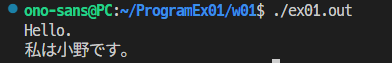
\includegraphics[scale=0.7]{img/wsl_result.png}
\caption{実行結果}
\label{result01}
\end{figure}

これは自分のWindows11のPCにWSL2を入れ, gccでコンパイルしたものだ.
1行目の「\texttt{Hello.}」はソースコード\ref{s01}の9行目,
「\texttt{printf("Hello.\textbackslash n");}」,
1行目の「\texttt{私は小野です。}」はソースコード\ref{s01}の10行目,
「\texttt{printf("私は小野です。\textbackslash n");}」,
にそれぞれ対応している.

\section{考察}

\subsection{\texttt{printf}の結合}

\texttt{printf}を2回に分けて文字を表示させているが,
繋げても表示できるのではないかと考え,
一つの\texttt{printf}で表した.

\begin{lstlisting}[caption=1つの\texttt{printf}で表したコード,label=]
#include <stdio.h>

int main(void)
{
    printf("Hello.\n私は小野です。\n"); // 1つのprintfに結合
    return 0;
}
\end{lstlisting}

表示された結果は頭\ref{result01}と同じような結果になった.

\subsection{\texttt{main}関数を\texttt{text}関数に変更}

\texttt{int main(void)}となっている部分を
\texttt{main}関数と呼ぶのであれば,
\texttt{main}の部分を\texttt{test}に変更し
\texttt{test}関数(?)にして実行してみた.

\begin{lstlisting}[caption=\texttt{main}を\texttt{test}に,label=]
#include <stdio.h>

int test(void) // main関数のmainの部分をtestに変更
{
    printf("Hello.\n");
    printf("私は小野です。\n");
    return 0;
}
\end{lstlisting}

コンパイルすると以下のように出力された.

\begin{figure}[H]
  \centering
  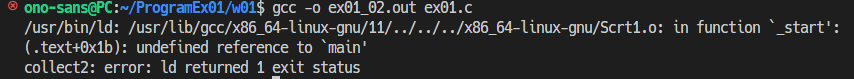
\includegraphics[scale=0.7]{img/error_main.png}
  \caption{実行結果}
  \label{result02}
\end{figure}

テキストに書き起こしたものを以下に載せる.

\begin{lstlisting}[caption=エラー文,label=]
ono-sans@PC:~/ProgramEx01/w01$ gcc -o ex01_02.out ex01.c
/usr/bin/ld: /usr/lib/gcc/x86_64-linux-gnu/11/../../../x86_64-linux-gnu/Scrt1.o: in function `_start':
(.text+0x1b): undefined reference to `main'
collect2: error: ld returned 1 exit status
\end{lstlisting}

エラーの内容を簡単に翻訳すると,
自分の入力したところとそこから1行目, 
3行目は自分が書いた内容との関連性はないと考えられる.
2行目を日本語に直すと「未定義の\texttt{main}への参照」となっていることから
簡単に言えば「\texttt{main}がないよ」と返されていることがわかる.

このことからC言語を実行するには\texttt{main}関数が不可欠で,
\texttt{main}以外の名前では認識されないと考えられる.

\cite{key1}より

\begin{itemize}
  \item \texttt{main}関数は必須.
  \item \texttt{main}関数から実行が開始される.
\end{itemize}

とのことから\texttt{main}関数があればそれ以外の関数も書くことができると
考えられる.
\clearpage
\subsection{\texttt{main}関数と\texttt{text}関数}
\texttt{printf}が上から実行されていったことから
\texttt{main}関数の下に\texttt{test}関数というものを書いてみる.

\begin{lstlisting}[caption=\texttt{main}関数と\texttt{text}関数,label=]
#include <stdio.h>

int main(void) // main関数
{
    printf("Hello.\n");
    return 0;
}

int main(void) // main関数
{
    printf("私は小野です。\n");
    return 0;
}
\end{lstlisting}

出力は以下の通りである.

\begin{figure}[H]
  \centering
  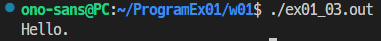
\includegraphics[scale=0.7]{img/main_test.png}
  \caption{実行結果}
  \label{result03}
  \end{figure}

図\ref{result01}のような結果を期待していたため,
予想通りにはならなかった.

ここから考えられることとして
恐らくコンパイラ側は機械語に翻訳する際
\texttt{main}関数の中身のみコンパイルしているもしくは
そこの部分のみ実行するようにしていると予想される.

\texttt{test}関数のような\texttt{main}関数以外の関数を使用する場合は
何か他の方法があるのだろうと考えられる.

\section{タイピング速度測定}
これが私の記録です.

\begin{figure}[H]
\centering
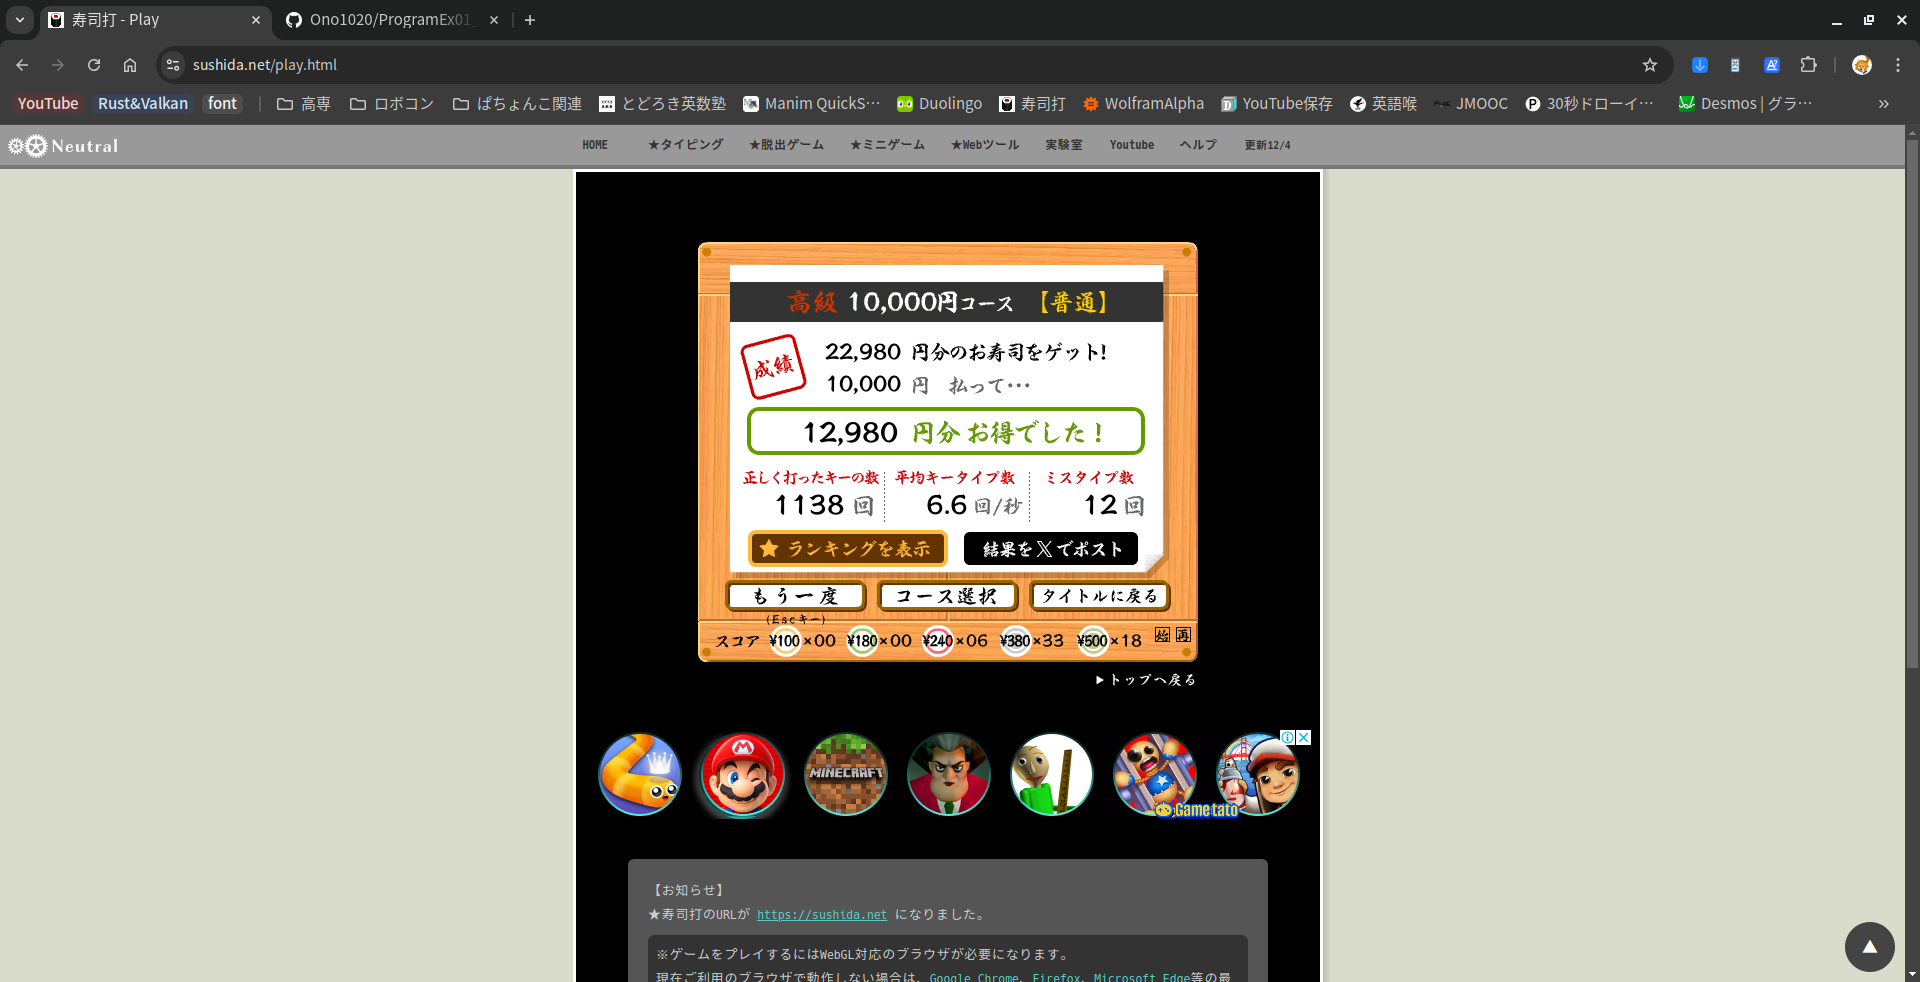
\includegraphics[scale=0.6]{img/sushida.png}

\caption{寿司打の記録}
\label{}
\end{figure}

\section{所感}
初めてのプログラミング演習ということで
初心に立ち返って授業を聞きましたが,
意外と抜けていた部分などもあったためとても勉強になりました.
レポートについても授業内で扱ったこと以外の知識はなるべく使わず,
新しいことをする場合は信頼性の高いサイトからの情報を使って,
「自分がここまでの知識しかもっていなかったとき, どのように考えるか」ということも
考えながら考察を書きました.

% 参考文献
\begin{thebibliography}{9} % 数字の最大の桁数分9追加
  % \bibitem{key1}example 工学基礎I\hspace{-1.2pt}I\hspace{-1.2pt}I
  \bibitem{key1}"Standard C++ Library Reference(日本語翻訳版)". IBM. ver.3.1.0. \url{https://www.ibm.com/docs/ja/zos/3.1.0?topic=functions-main-function}, (\today).
\end{thebibliography}
\end{document}